\documentclass[a4paper,10pt]{article}

%\usepackage{natbib}
\usepackage{amsthm}
\usepackage{amsfonts}
\usepackage{amssymb}
\usepackage{amsmath}
\usepackage{latexsym}
\usepackage{graphicx}
\usepackage[]{algorithm2e}

\usepackage{doc}

\newtheorem*{theorem}{Theorem}
\theoremstyle{definition}
\newtheorem*{definition}{Definition}

\hoffset -1in \topmargin 0mm \voffset 0mm \headheight 0mm
\headsep0mm
\oddsidemargin  20mm     %   Left margin on odd-numbered pages.
\evensidemargin 20mm     %   Left margin on even-numbered pages.
\textwidth   170mm       %   Width of text line.
\textheight  252mm

\makeatletter
\renewcommand\@openbib@code{%
     \advance\leftmargin  \z@ %\bibindent
      \itemindent \z@
     % Move bibitems close together
     \parsep -0.8ex
     }
\makeatother

\makeatletter
\renewcommand\section{\@startsection {section}{1}{\z@}%
                                   {-3.5ex \@plus -1ex \@minus -.2ex}%
                                   {1.5ex \@plus.2ex}%
                                   {\large\bfseries}}
\makeatother

\makeatletter
\renewcommand\subsection{\@startsection {subsection}{1}{\z@}%
                                   {-3.5ex \@plus -1ex \@minus -.2ex}%
                                   {1.5ex \@plus.2ex}%
                                   {\normalsize\bfseries}}
\makeatother

\makeatletter
	\setlength{\abovecaptionskip}{3pt}   % 0.25cm 
	\setlength{\belowcaptionskip}{3pt}   % 0.25cm 
\makeatother

\begin{document}
\pagestyle{empty}

\begin{center}
{\bf \Large RUNTIME ANALYSIS OF EVOLUTIONARY ALGORITHM\\
\medskip GENERATING TESTS FOR THE DIJKSTRA ALGORITHM}
\end{center}

\smallskip
\begin{center}
{\large Denis Antipov and Maxim Buzdalov}
\end{center}

\smallskip
\begin{center}
ITMO University\\
Computer Technology Department\\
49, Kronverkskiy pr., Saint-Petresburg \\
Russia\\
antipovden@yandex.ru, mbuzdalov@gmail.com
\end{center}

\bigskip
\noindent Abstract: \textit{This article describes the theoretical analysis of expected runtime of the evolutionary algorithm that generates tests for the Dijkstra algorithm. The proof of the upper bound is shown for the case of rarefied graphs. Also some ideas of the proof of the upper bound for the dense graphs are given here.}

\vspace*{10pt} \noindent Keywords: \textit{Evolutionary algorythms, runtime analysis, test generation.}

\bigskip
\section{Introduction}
\label{sec:1}

Evolutionary algorithms form a class of optimization algorithms that use ideas of the natural evolution. Ususally this algorithms can be described in the following way:
\begin{itemize}
 \item At first step the algorithm generates the initial group (population) of potential solutions.
 \item On every iteration of the algorithm the population is changed with the operators of mutaton and crossover.
 \item Algorithm is finished when it finds the solution good enough or when it perfoms maximum allowed number of iterations.
\end{itemize}

Such algorithms usually don't find optimal solution, but they can find good solutions in a short period of time. That's why they are good for the problem of test generation \textbf{REFERENCE}. But runtime analysis of the evolutionary algorithms that generate tests hasn't been perfomed yet. 

The theoretical analysis of the evolutionary algorithms usually helps to find their weak parts. Modification of the algorithms with this knowledge can improve the expected runtime of the algorithms \textbf{REFERENCE to the Dojerr's ONEMAX crossover}.

So to start the runtime analysis of the evolutionary algorythms that generate tests we've chosen the algorithm that generates the directed graph with real weights for the Dijkstra algorithm.

Let us show you the structure of this article. In the second section we will introduce the analysed algorithm in details. In the third section we will show the upper bound on runtime in the case of rarefied graphs. Next, in the fourth section we will show our ideas of analysis for the case of dense graphs. In the fifth section we will show the correlation of the theoretical results with the results of the experiments. Finally in conclusion we will sum up the results and discuss the further ways of work.


\section{Problem Formulation}
\label{sec:2}

The algorithm to be analysed is quite simple. It tries to find such directed graph with real weights that Dijkstra algorithm run on this graph will relax all it's edges. 
Input of the algorithm is two integer numbers: $V$ and $E$ -- number of vertices and number of edges in the graph. At first it generates random graph with $V$ vertices and $E$ edges and edges weights in the interval $[0; 1]$. Then it calculates $f$ -- number of edges relaxed by the Dijkstra algorithm. Here we should notice that our implementation of Dijkstra algorithm iterates through the edges form current vertex in the order in which edges have been given it on input, so the number of relaxed edges for each pair of vertices can be greater than one. 

After that algorithm mutates current graph and calculates it's number of relaxed edges $f'$. If $f' \ge f$ then current graph is replaced with the new one. Algorithm repeats mutations until it finds graph with all edges relaxed. We use simple RMHC mutation: we delete one random edge and add one edge with random start and end vertices and random weight in the interval $[0; 1]$.

The pseudocode of the algorithm is presented on the figure~\ref{pseudocode}. Function $dijkstra(graph)$ returns the number of the relaxed edges in the $graph$.

\begin{figure}[ht]
\begin{center}
\begin{algorithm}[H]
  \KwData{$V$, $E$}
  \KwResult{$graph$ with all edges relaxed}
  
  $graph \gets init()$
  
  $f \gets dijkstra(graph)$
  
  \While{$f \ne E$}{
    
    $graph' \gets mutate(graph)$
    
    $f' \gets dijkstra(graph')$
    
    \If{$f' \ge f$}{
      $graph, f \gets graph', f'$
    }
  }
 % \Return{$graph$}
  \end{algorithm}
  \caption{Pseudocode of the analysed algorithm}
  \label{pseudocode}
 \end{center}
\end{figure}

\section{Upper bound for the rarefied graph}
\label{sec:3}

Let's consider the case when $V \gg E$. In this case if we've relaxed edge, then with high probability we've put it from current connected component outward it. So we can modify our algorithm: it will accept new graph only if it's fitness not less then previous' one and if all the edges that has been mutaded during the algorithm form a tree with a root in the start vertex. Also the initial graph will be the worst case graph: all the edges will be loops from starting vertex back to itself. It will slowdown the algorithm because it won't increase fitness value when it can do it. But it's easier to find the exact expected runtime of this modification that will be upper bound for the original algorithm.

Let $p_{ur}(i)$ be the probability to change the edge that hasn't been relaxed when the current fitness equals to $i$. Also let $p_{sr}(i)$ ad $p_{eu}(i)$ be the probabilities to choose the vertex reachable from the starting one as the start of the edge and the unreachable vertex as the end.
 Then the probability to encrease the fitness by one will be:
 
 $$ p_{+1}(i) = p_{ur}(i) \cdot p_{sr}(i) \cdot p_{eu}(i) = \frac{E - i + 1}{E} \cdot \frac{i}{V} \cdot \frac{V - i}{V}$$
 
 If $V > E + 1$ then the expected runtime of the algorithm could be written in the next way:
 
 \begin{align*}
  T & = \sum_{i = 1}^E \frac{1}{p_{+1}(i)} = \sum_{i = 1}^E \frac{EV^2}{i(V - i)(E - i + 1)} = \\
    & = EV \sum_{i = 1}^E \frac{1}{E - i + 1} \left(\frac{1}{i} + \frac{1}{V - i} \right) = \\
    & = EV \sum_{i = 1}^E \left[ \frac{1}{E + 1} \left( \frac{1}{E - i + 1} + \frac{1}{i}\right) + \frac{1}{V - E - 1} \left( \frac{1}{E - i + 1} - \frac{1}{V - i} \right)\right] = \\
    & = \left( \frac{2EV}{E + 1} + \frac{EV}{V - E - 1}\right) \sum_{i = 1}^E \frac{1}{i} - \frac{EV}{V - E - 1} \sum_{i = 1}^E \frac{1}{V - i} \approx \\
    & \approx \frac{EV(2V - E - 1)}{(E + 1)(V - E - 1)}(\gamma + \ln{E}) - \frac{EV}{V - E - 1} \ln \frac{V - 1}{V - E}
 \end{align*}
 
 where $\gamma$ is Euler's constant. If $V = E + 1$ the runtime of the algorithm begins to quadratically depend on the number of edges:
 
 \begin{align*}
  T & = 2E \sum_{i = 1}^E + E(E + 1) \sum_{i = 1}^E \frac{1}{i^2} \approx 2E(\gamma + \ln{E}) + E(E + 1)(\frac{\pi^2}{6} + o(1)) = \\
    & = \frac{\pi^2 E^2}{6} + o(\frac{\pi^2 E^2}{6})
 \end{align*}

 This result is much higher then experiments results, so for the cases when $V > E$ but $V \approx E$ we need some other analysis.
 
 Finally for the rarefied graphs let's consider case when $V = aE$ where $a$ is some constant greater then one. Then the equality for runtime turns into:
 
 \begin{align*}
  T & = \frac{aE^2(2aE - E - 1)}{(E + 1)(aE - E - 1)} (\ln{E} + \gamma) - \frac{aE^2}{aE - E - 1} \ln \frac{aE - 1}{(a - 1) E} \approx \\
    & \approx \frac{aE}{(a - 1)} \left((2a - 1)(\ln{E} + \gamma) - \ln\frac{a}{a - 1} \right)\approx \\
    & \approx aE(\ln{E} + \gamma) \frac{2a - 1}{a - 1} = V(\ln{E} + \gamma)\left(2 + \frac{1}{a - 1}\right)
 \end{align*}

\section{Dense graphs analysis}
\label{sec:4}

The analysis shown above can't be applied to the cases when $V \le E$ because the slower modification of the algorithm can't acept graphs with $f \ge V$ because it accepts only trees. So let's consider the graph with two vertices and $E$ edges at first. As we has noticed, the Dijkstra algorithm iterates through the edges in the order they were given on input. It means that in graphs with two vertices relaxed edges will be ordered by decreasing weight. So we can consider them as in the figure~\ref{edges}. 

\begin{figure}[ht]
\begin{center}
  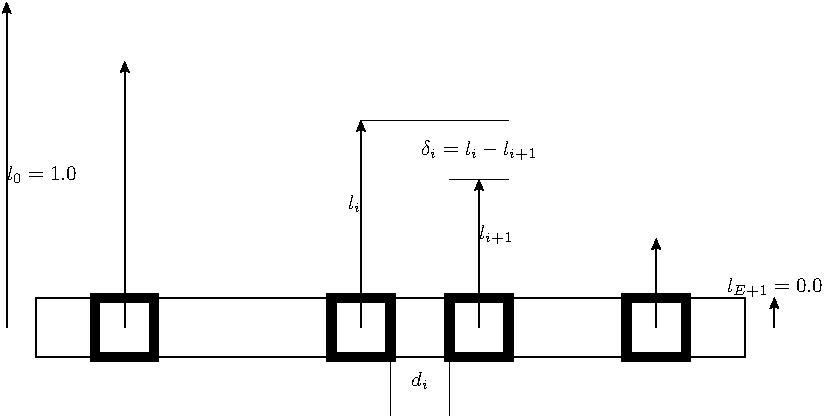
\includegraphics[width=12cm]{pic/edges.pdf}
  \caption{Array of edges. Bold sqares mark the relaxed edges. Vertical arrows show their weight.}
  \label{edges}
 \end{center}
\end{figure}

Let $d_i$ be the number of unrelaxed edges between $i$-th and $i + 1$-th relaxed edges. Also let $\delta_i$ be the difference of their weights. For the correctness of this definition let's add one relaxed edge with weight $1$ to the beginning of the array and one relaxed edge with weight $0$ to it's end.

It means that the probability to relax an unrelaxed edge in the case of it's mutation won't be less then production of the probability to give this edge right orientation and the probability to give it weight between the weights of the next and previous relaxed edges:
$$p_\text{relax}(edge) \ge \frac{1}{4} \cdot \delta_{i(edge)}$$
where $i$ is the number of interval between relaxed edges where the unrelaxed edge locates. So the full probability to increase fitness will be
$$p_{+1} \ge \sum_{e - \text{unrelaxed}} \frac{1}{4E} \delta_{i(e)} =  \frac{1}{4E}\sum_{i = 0}^{f} d_i \delta_i$$

But there is possible situation when we mutate a relaxed edge. If it has happened, the mutated edge must be oriented in the same direction and must have new weight between the weights of the next and previous relaxed edges for acceptance of new graph. The probability of this case is
$$p_\text{change} = \sum_{i = 1}^f \frac{1}{4E} (\delta_{i - 1} + \delta_i) = 2 - \delta_0 - \delta_f$$

This event also can cause the ``opening'' of another edges that will be relaxed. For example, if we've encreased the weight of the relaxed edge and there was an unrelaxed edge just after it that was oriented from the starting vertex to another one and had a weight just a little greater then the relaxed edge. But if we ignore this case in our analysis, the found upper bound will be greater then the real one, because this cases increase fitness and speed up the algorithm.

Actually we are interested in the event of mutating relaxed edge because it changes $\delta_i$ and $\delta_{i - 1}$. So we can write the inequation to find the expected time of increasing number of the relaxed edges by one for the specified set of $\{d_i\}$ and $\{\delta_i\}$:

\begin{align*}
T(\{d_i\}_{i = 0}^f, \{\delta_i\}_{i = 0}^f) & \le \sum_{i = 0}^f \frac{1}{4E}d_i \delta_i + \\
& + \sum_{i = 1}^f \frac{1}{4E} \int\limits_{0}^{\delta_i + \delta_{i - 1}} (1 + T(\{d_j\}_{j = 0}^f, \{\delta_0, ... \delta_{i-1} + \delta_i - l, l, ...\delta_f\}) ) dl + \\
& + \left(1 - \sum_{i = 0}^f \frac{1}{4E}d_i \delta_i - \sum_{i = 1}^f \frac{1}{4E}(\delta_{i - 1} + \delta_i) \right)(1 + T(\{d_i\}_{i = 0}^f, \{\delta_i\}_{i = 0}^f)) \\
\end{align*}

From where we can get:

\begin{align}
 T(\{d_i\}_{i = 0}^f, \{\delta_i\}_{i = 0}^f) \le \frac{4E + \sum_{i = 1}^f\int\limits_{0}^{\delta_i + \delta_{i - 1}} T(\{d_j\}_{j = 0}^f, \{\delta_0, ... l ...\delta_f\})  dl}{\sum_{i = 0}^f d_i \delta_i + \sum_{i = 1}^f (\delta_{i - 1} + \delta_i)} \label{runtime_inequation}
\end{align}

Let $I_i(\delta_0, ... \delta_{i - 2}, \delta_{i + 1} ...\delta_f)$ be $\int\limits_{0}^{\delta_i + \delta_{i - 1}} T(\{d_j\}_{j = 0}^f, \{\delta_0, ... l ...\delta_f\})  dl$. In other words using~\ref{runtime_inequation} we can say:
\begin{align*}
I_i(\delta_0, ... \delta_{i - 2}, \delta_{i + 1} ...\delta_f) \le \int\limits_{0}^{\delta_i + \delta_{i - 1}} \frac{4E + \sum_{j = 1}^f I_j(\delta_0, ... \delta_{i - 2}, \delta_i + \delta_{i - 1} - l, l, \delta_{i + 1} ...\delta_f)  dl}{\sum_{i = 0}^f d_i \delta_i + \sum_{i = 1}^f (\delta_{i - 1} + \delta_i)} dl
\end{align*}

It gives us a system of differential inequations. For $f = 0$ the solution is simple:

$$T(\{E\}, \{1\}) \le \frac{4E}{E} = 4$$

For $f = 1$ there is only $I_1$ that doesn't depend on any $\delta_i$:

$$I_1 \le \int\limits_0^1 \frac{4E + I}{d_0(1 - l) + d_1 l + 1} dl$$

From where we can find $I_1$ and later $T(d_0, d_1, \delta_0, \delta_1)$:

$$I_1 \le \frac{4E\ln\frac{d_1 + 1}{d_0 + 1}}{d_1 - d_0 - \ln\frac{d_1 + 1}{d_0 + 1}}$$

$$T(d_0, d_1, \delta_0, \delta_1) \le \frac{4E \frac{d_1 - d_0}{d_1 - d_0 - \ln\frac{d_1 + 1}{d_0 + 1}}}{d_0\delta_0 + d_1\delta_1 + 1}$$

From the inequation above we can see that the worst case for the $T(d_0, d_1, \delta_0, \delta_1)$ is when $\delta_i$ for the lager $d_i$ is $0$. Also we can show that the  worst case is when $d_0$ or $d_1$ is $0$ by differentiating $T$ by the minor $d_i$. The derivative will have one sign for every minor $d_i$ from $0$ to $\lfloor\frac{E - 1}{2}\rfloor$ and maximum of $T$ will be:

$$ T_\text{worst} = T(E - 1, 0, 0, 1) = \frac{E - 1}{E - 1 - \ln(E - 1)} $$

For greater $f$ there is a system of $(f - 1)^2$ differential equations for $f - 1$ functions of $f - 1$ arguments. The solution of this system hasn't been found yet, but authors belive that the expected time of increasing the number of relaxed edges isn't greater then $4E^2$ for every $f$. It will give us the upper bound for the expected runtime $4E^3$ because fitness can't increase more then $E$ times.

\section{Experiments}
\label{sec:5}

Some series of experiments have been performed. Most of them gathered different statistics about graphs during algorithm run and gave us idea of the algorithm modification described in the section~\ref{sec:3}. Also we performed experiments that approved upper bound on runtime for the rarefied graphs. Figure~\ref{exper_rar} shows the results for $E = 100$ and $V$ from $110$ to $1000$ with step $10$ and $100$ runs for each value. As we can see, the upper bound is strongly above the experiments result, but it's not far above them.

\begin{figure}[ht]
 \begin{center}
  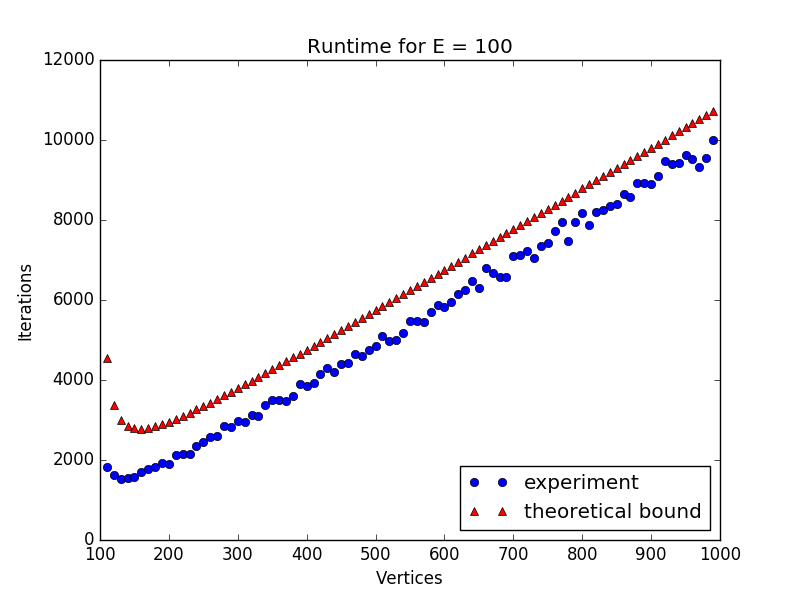
\includegraphics[width = 11cm]{pic/exper_rar.png}
  \caption{Experiment results for the rarefied graphs}
  \label{exper_rar} 
 \end{center} 
\end{figure}

Also we perfomed experiments for the dense graph with two vertices. We ran our algorithm for $V = 2$ and $E$ from $2$ to $98$ with step $3$ $80$ times for each value. Results approved our assumption that total runtime of the algorithm is not greater then $4E^3$. The results are shown in the figure~\ref{exper_den}.

\begin{figure}[ht]
 \begin{center}
  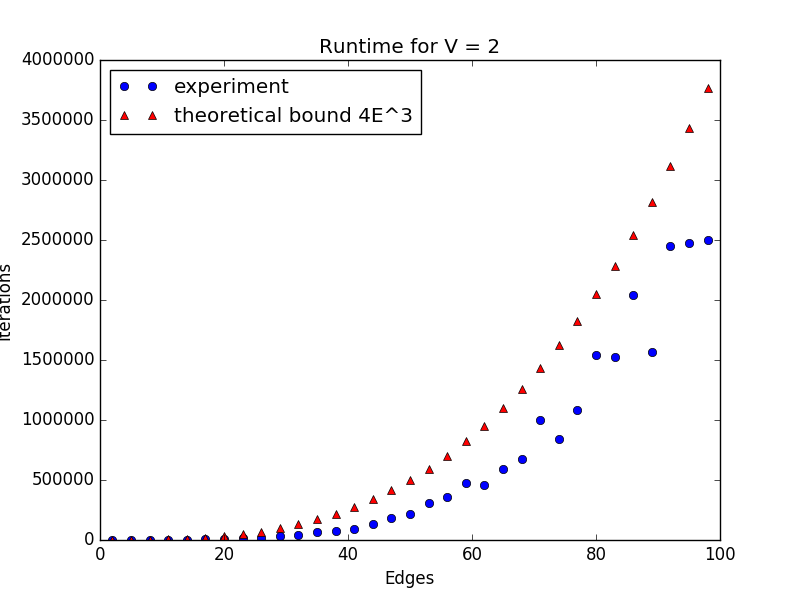
\includegraphics[width = 11cm]{pic/exper_den.png}
  \caption{Experiment results for the dense graphs}
  \label{exper_den} 
 \end{center} 
\end{figure}

\section{Conclusion}
\label{sec:6}

In this paper we showed the analysis of the expected runtime of evolutionary algorithm that generates tests for the Dijkstra algorithm. We've found upper bound on runtime for the case of dense graphs and approved it with experiments. Also we've described ideas of finding bound to the dense graph with two vertices. In the nearest future we are going to find exact bound for this case by solving the systems of differential equations. Also we are going to spread this proof on the case of dense graphs with more then two vertices.

\end{document}
